\documentclass[12pt]{article}
\usepackage[top=1in, bottom=1in, left=.75in, right=.75in]{geometry}
\usepackage{amsmath}
\usepackage{fancyhdr}
\usepackage{graphicx}
\usepackage{txfonts}
\usepackage{multicol,coordsys}
\usepackage[scaled=0.86]{helvet}
\renewcommand{\emph}[1]{\textsf{\textbf{#1}}}
\usepackage{anyfontsize}
% \usepackage{times}
% \usepackage[lf]{MinionPro}
\usepackage{tikz,pgfplots,mathrsfs}
%\def\degC{{}^\circ{\rm C}}
\def\ra{\rightarrow}
\usetikzlibrary{calc, backgrounds}
\pgfplotsset{compat = newest}
\newcommand{\blank}[1]{\rule{#1}{0.75pt}}

\pgfplotsset{my style/.append style={axis x line=middle, axis y line=
middle, xlabel={$x$}, ylabel={$y$},axis equal}}

%yticklabels={,,} , xticklabels={,,}

% \setmainfont{Times}
% \def\sansfont{Lucida Grande Bold}
\parindent 0pt
\parskip 4pt
\pagestyle{fancy}
\fancyfoot[C]{\emph{\thepage}}
\fancyhead[L]{\ifnum \value{page} > 1\relax\emph{Math 251: Final Exam}\fi}
\fancyhead[R]{\ifnum \value{page} > 1\relax\emph{13 Dec 2022}\fi}
\headheight 15pt
\renewcommand{\headrulewidth}{0pt}
\renewcommand{\footrulewidth}{0pt}
\let\ds\displaystyle
\def\continued{{\emph {Continued....}}}
\def\continuing{{\emph {Problem \arabic{probcount} continued....}}\par\vskip 4pt}


\newcounter{probcount}
\newcounter{subprobcount}
\newcommand{\thesubproblem}{\emph{\alph{subprobcount}.}}
\def\problem#1{\setcounter{subprobcount}{0}%
\addtocounter{probcount}{1}{\emph{\arabic{probcount}.\hskip 1em(#1)}}\par}
\def\subproblem#1{\par\hangindent=1em\hangafter=0{%
\addtocounter{subprobcount}{1}\thesubproblem\emph{#1}\hskip 1em}}
\def\probskip{\vskip 10pt}
\def\medprobskip{\vskip 2in}
\def\subprobskip{\vskip 45pt}
\def\bigprobskip{\vskip 4in}

\begin{document}
{\emph{\fontsize{26}{28}\selectfont Math F251\hfill
{\fontsize{32}{36}\selectfont Final Exam}
\hfill Fall 2022}}
\vskip 2cm
\strut\vtop{\halign{\emph#\hskip 0.5em\hfil&#\hbox to 2in{\hrulefill}\cr
\emph{\fontsize{18}{22}\selectfont Name:}&\cr
\noalign{\vskip 10pt}}}
%%\emph{\fontsize{18}{22}\selectfont Student Id:}&\cr
%%\noalign{\vskip 10pt}
%%\emph{\fontsize{18}{22}\selectfont Calculator Model:}&\cr
%}}
%\hfill
%\vtop{\halign{\emph{\fontsize{18}{22}\selectfont #}\hfil& \emph{\fontsize{18}{22}\selectfont\hskip 0.5ex $\square$ #}\hfil\cr
%Section: & 001 (Jill Faudree)\cr
%\noalign{\vskip 4pt}
%         & 002 (James Gossell)\cr
%\noalign{\vskip 4pt}
%         & 005 (James Gossell)\cr}}

\vfill
{\fontsize{18}{22}\selectfont\emph{Rules:}}

You have 2 hours to complete the final exam.  

Partial credit will be awarded, but you must show your work.

You may have a single handwritten $3 \times 5$ notecard.

Calculators are not allowed. 


Place a box around your  \fbox{FINAL ANSWER} to each question where appropriate.

%If you need extra space, you can use the back sides of the pages.
%Please make it obvious  when you have done so.

Turn off anything that might go beep during the exam.

Good luck!
\vfill
\def\emptybox{\hbox to 2em{\vrule height 16pt depth 8pt width 0pt\hfil}}
\def\tline{\noalign{\hrule}}
\centerline{\vbox{\offinterlineskip
{
\bf\sf\fontsize{18pt}{22pt}\selectfont
\hrule
\halign{
\vrule#&\strut\quad\hfil#\hfil\quad&\vrule#&\quad\hfil#\hfil\quad
&\vrule#&\quad\hfil#\hfil\quad&\vrule#\cr
height 3pt&\omit&&\omit&&\omit&\cr
&Problem&&Possible&&Score&\cr\tline
height 3pt&\omit&&\omit&&\omit&\cr
&1&&8&&\emptybox&\cr\tline
&2&&8&&\emptybox&\cr\tline
&3&&8&&\emptybox&\cr\tline
&4&&10&&\emptybox&\cr\tline
&5&&10&&\emptybox&\cr\tline
&6&&10&&\emptybox&\cr\tline
&7&&16&&\emptybox&\cr\tline
&8&&12&&\emptybox&\cr\tline
&9&&12&&\emptybox&\cr\tline
&10&&6&&\emptybox&\cr\tline
&Extra Credit&&5&&\emptybox&\cr\tline
&Total&&100&&\emptybox&\cr
}\hrule}}}

\newpage
\begin{enumerate}
%%% straight limits
\item (8 points) Evaluate the limits. An answer without clear, mathematically precise work, will not earn full credit. Any use of L'H\^{o}pital's Rule should be indicated using an \textbf{H} over the equal sign.
	\begin{enumerate}
	\item $\displaystyle \lim_{x \to -4} \frac{\frac{1}{4}+\frac{1}{x}}{x+4}$
	\vfill
	\item $\displaystyle \lim_{x \to -1^+} \frac{8+x^2}{x^2-1}$
	\vfill
	\end{enumerate}
\newpage
%%% straight derivatives
\item (8 points) Find the derivative. You do not need to simplify your answer.
	\begin{enumerate}
	\item $\displaystyle B(x)=\frac{\tan(2x)}{{x^2+16}}$
	\vfill
	\item $\displaystyle f(x)=e^{-x}+\frac{1}{x}+\sqrt{2x}$
	\vfill
	\end{enumerate}
%%% straight integrals
\item (8 points) Evaluate the integrals. You do not need to simplify your answer.
\begin{enumerate}
	\item $\displaystyle \int (4\sin(x)+8x^3-1)\, dx$
	\vfill
	\item $\displaystyle \int_0^2 \pi x \sqrt{x^2+9} \, dx $
	\vfill
	\end{enumerate}
\newpage
%%% implicit differentiation & tangent line
\item (10 points) Below is the graph of $x^2-2xy+y^3=8.$\\
\includegraphics[scale=.25]{implicit-graph.png}

(a) Use implicit differentiation to find $\displaystyle \frac{dy}{dx}.$
\vfill
(b) Find an equation of the line tangent to the curve $x^2-2xy+y^3=8$ when $x=0.$
\vfill
(c)  On the graph above, sketch the tangent line found in part (b).
\vspace{.5in}
\newpage
%%% optimization
\item (10 points) A farmer has 900 meters of fencing with which to build two adjacent rectangular pens. One side of the enclosed area borders a river and does not require fencing. (See figure below.) Determine the largest total area that can be enclosed by the two pens.\\
You must show your work, use calculus to justify your answer. Your final answer should be a sentence and should include units.\\

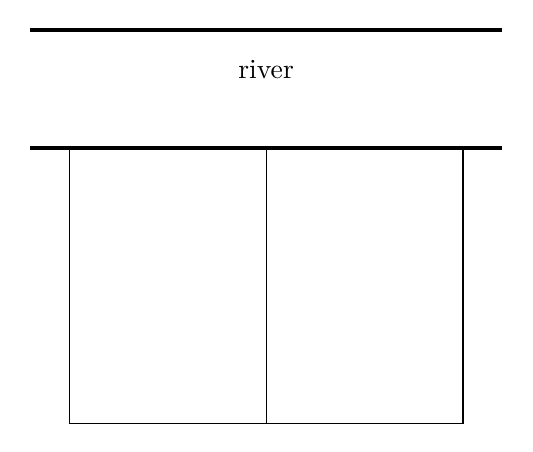
\begin{tikzpicture}
\draw[ultra thick] (-3,5)--(3,5);
\node at (0,4.5){river};
\draw[ultra thick] (-3,3.5)--(3,3.5);
\draw (-2.5,3.5)--(-2.5,0)--(2.5,0)--(2.5,3.5)(0,0)--(0,3.5);
\end{tikzpicture}
\vfill
Did you ....\\
$\square$ Include a clear justification?\\
$\square$ Answer the question?\\
\newpage
%%% initial value problem & average velocity
\item (10 points) Assume the acceleration of an object is given by $a(t)=12t-2$ on the interval $[0,60]$ where $t$ is measured in seconds  and $a(t)$ is measured in meters per second per second (i.e. $m/s^2$).\\
\begin{enumerate}
\item If the initial velocity of the object is $10$ meters per second, find the velocity function of the object, $v(t).$
\vfill
\item If $s=0$ when $t=0,$ find an equation modeling the position of the object, $s(t).$
\vfill
\item Determine the average velocity of the object in the first 3 seconds.
\vfill
\end{enumerate}

\newpage
%%%% sketch the shape of the graph
\item (16 points) Use the axes below to sketch a graph of a function $g(x)$ that satisfies \emph{all} of the conditions in the bulleted list. Make sure to label any asymptotes, minimums or maximums, and inflection points. (See check list.)

\begin{minipage}{0.7\textwidth}
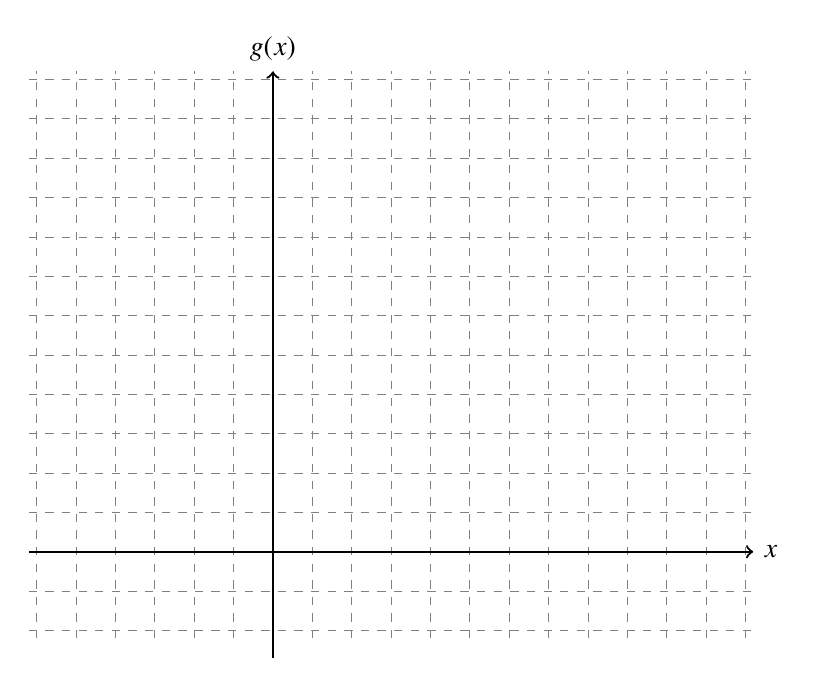
\begin{tikzpicture}[scale=0.5]
	\draw [help lines,dashed] (-6.2,-2.2) grid (12.2,12.2);
	\draw [thick, ->] (-6.2,0)--(12.2,0) node[right] {$x$};
	\draw [thick, ->] (0,-2.7)--(0,12.2) node[above]{$g(x)$};
	\end{tikzpicture}
\end{minipage}
\hspace*{-1in}
\begin{minipage}{0.4\textwidth}
\begin{itemize}
\item $g(x)$ is continuous on its domain $(-\infty,6) \cup (6,\infty).$
\item $g(1)=5$, $g''(1)=0$
\item $g(3)=2,$ $g'(3)=0$
\item $\displaystyle \lim_{x \to 6} g(x)=\infty$
\item $\displaystyle \lim_{x \to -\infty} g(x)=9$
\item $g'(x)>0$ on $(3,6)$ and $g'(x)<0$ on $(-\infty,3)\cup(6,\infty)$
\item $g''(x)>0$ on $(1,6) \cup (6,\infty) $ and $g''(x)<0$ on $(-\infty,1)$
\end{itemize}
\end{minipage}
\vfill
Did you ....\\
$\square$ label any asymptotes with its equation?\\
$\square$ label any maximums or minimums with \emph{local min, local max, absolute min,} or \emph{absolute max}?\\
$\square$ label any inflection points with \emph{inflection point}?\\
\newpage
%%%% Net Change
\item (12 points) Let $r(t)$ denote that rate at which a thick sheet of volcanic lava cools where $r$ is measured in degrees Fahrenheit per day and $t$ is measured in days. 
\begin{enumerate}
\item Write a complete sentence explaining $r(10)=-20$ in the context of the problem. Include units in your answer. 
\vfill
\item Explain why you would expect $r(t) < 0.$
\vfill
\item Write a complete sentence explaining $\int_0^{30} r(t) \, dt = -420$ in the context of the problem. Include units in your answer. 
\vfill
\item Assume the lava began with a temperature of $2080^oF.$ Write an expression for the temperature of the lava a year later.
\vfill
\end{enumerate}

\newpage
%%%% FTC P1 & friends
\item (12 points) Consider the function $f(x)$ with domain $[0,9]$ graphed below. 

\begin{center}
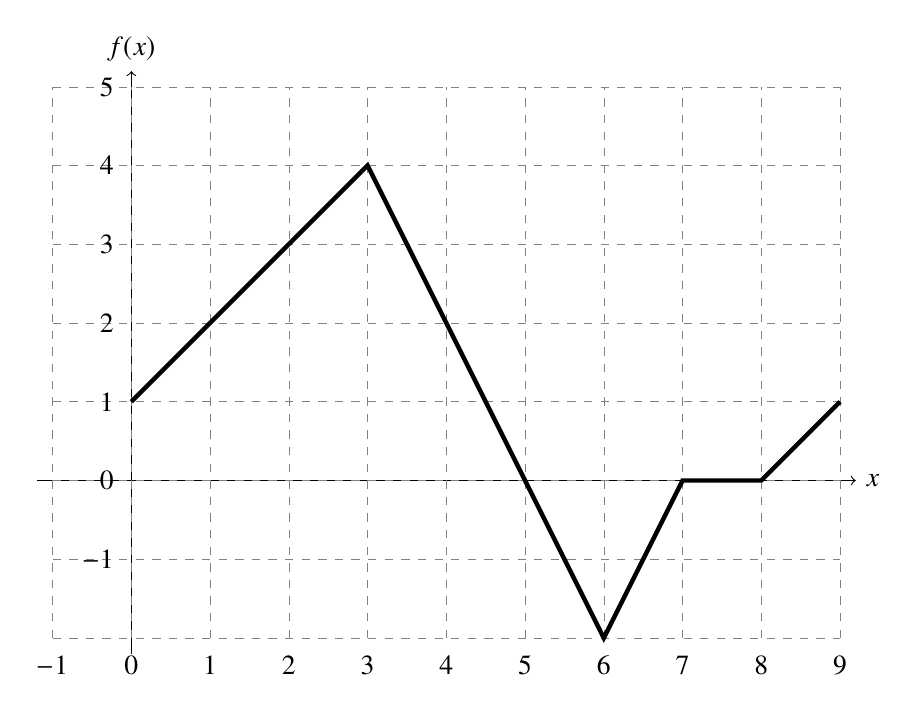
\begin{tikzpicture}[scale=1]
\draw[->] (-1.2,0) -- (9.2,0) node[right] {$x$};
\draw[->] (0,-2.2) -- (0,5.2) node[above] {$f(x)$};
\draw[help lines, dashed] (-1,-2) grid (9,5);
\draw[style= ultra thick] (0,1) --  (3,4) --(6,-2)--(7,0)--(8,0)--(9,1);
%\draw[style= ultra thick] (0,0) arc (180:0:1) -- (4.2,1.1);
\foreach \x in {-1,0,1,2,3,4,5,6,7,8,9}
\draw (\x,-2.1) node[below] {$\x$};
\foreach \y in {-1,0,1,2,3,4,5}
\draw (-0.1,\y) node[left] {$\y$};
\end{tikzpicture}
\end{center}

\bigskip
\begin{enumerate}
\item What is the value of $f(2)$?

\vfill

\item  What is the value of $f'(2)$?

\vfill

\item  Evaluate $\displaystyle \int_{0}^{9} f(x)\,dx$.

\vfill

\item Let $H(x) =\ds \int_0^x f(s)\,ds$.  What is the value of $H(4)$?

\vfill

\item  For $H(x)$ from part \textbf{d.}, what is the value of $H'(4)$.

\vfill

\item For $H(x)$ from part \textbf{d.}, over what interval is $H(x)$ decreasing?
\vfill
\end{enumerate}

\newpage
%meaning of asymptote and roc
\item (6 points) Let $\displaystyle f(t)= \frac{300e^{2t}+100t}{e^{3t} +1}$ denote the rate of change of a population of fruit flies where $t$ is measured in days and $f$ is measured in fruit flies per day.\\
\begin{enumerate}
\item Evaluate $\displaystyle \lim_{t \to \infty} f(t).$ You must show your work to receive full credit.
\vfill
\item Explain, using complete sentences, what your calculation in part (a) indicates about the \textbf{population} of fruit flies. Your answer should reference the value you obtained in part (a).
\vfill
\end{enumerate}
\end{enumerate}
\newpage
%%% Extra Credit Newton's Method
\textbf{Extra Credit} (5 points) The graph of the function $f(x)=x^2-\ln(3x)$ is shown.

%\vskip -.7in

\begin{minipage}{0.5\textwidth}

	\subproblem{}
	Suppose Newton's method is used to find an approximate solution to
	$f(x)=0$ from an initial guess of $x_1=2$. Sketch on the graph how the
	next approximation $x_2$ will be found, labeling
	its location on the $x$-axis.
	%\vskip 1.in
\end{minipage}
\begin{minipage}{0.5\textwidth}

\hfill
	\pgfplotsset{my style/.append style={axis x line=middle, axis y
			line=middle, xlabel={$x$}, ylabel={$y$}}}
	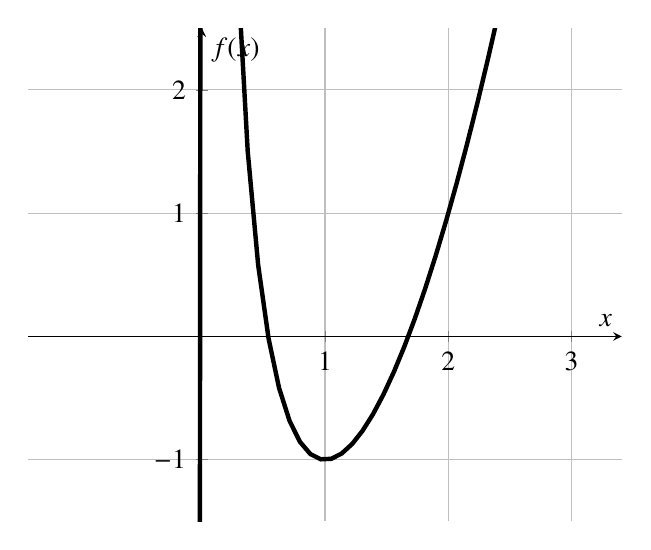
\begin{tikzpicture}
	\begin{axis}[scale=1.1, my style, xtick={ 0,...,2,3}, ytick={-3,...,3},
	xmin=-.5, xmax=2.5, ymin=-1.5, ymax=2.5, minor y tick num=0,
	minor x tick num=0, mark size=5.0pt,
	grid=both, ylabel=$f(x)$,samples=60]
	\addplot[domain=-2:3, -, ultra thick] {x^2+2/x -4};
	\end{axis}
	\end{tikzpicture}
\end{minipage}

\bigskip
\subproblem{} For $x_1=2$, give a formula for $x_2$. You do not need to
simplify, but your answer should be in a form where a calculator
would compute a numerical value.

\vfill

\vspace{1.0in}


\end{document}
